\documentclass[a4paper,UKenglish,cleveref,autoref]{oasics-v2021}

% Manuscript v0.15.1, deployed-meter figure and corrected artifact delivery, 2026-10-09.
% Native reconstruction and all-15-run FP16 summaries are the manuscript basis.
\hideOASIcs
\usepackage{booktabs}
\usepackage{array}
\usepackage{tabularx}
\usepackage{xcolor}
\usepackage{placeins}
\renewcommand{\orcidsymbol}{
\includegraphics[height=9pt]{orcid.pdf}}
% Suppress the empty publisher ribbon in the author version.
\makeatletter
\let\@oddfoot\@empty
\makeatother
\setlength{\textfloatsep}{14pt plus 2pt minus 2pt}
\setlength{\floatsep}{10pt plus 2pt minus 2pt}
\setlength{\intextsep}{10pt plus 2pt minus 2pt}
\renewcommand{\topfraction}{0.95}
\renewcommand{\bottomfraction}{0.90}
\renewcommand{\textfraction}{0.05}
\renewcommand{\floatpagefraction}{0.85}
\setcounter{topnumber}{3}
\setcounter{totalnumber}{4}
\newcolumntype{L}[1]{>{\raggedright\arraybackslash}p{#1}}
\newcolumntype{R}[1]{>{\raggedleft\arraybackslash}p{#1}}
\newcolumntype{Y}{>{\raggedright\arraybackslash}X}

\bibliographystyle{plainurl}
\graphicspath{{figures/}}

\newcommand{\urecs}{u.RECS}
\title{How Fast Is Fast Enough? Reference-Calibrated Energy Measurement for Edge-AI Inference}
\titlerunning{Reference-Calibrated Energy Measurement for Edge-AI Inference}

\author{Kevin Mika}
{CITEC -- Bielefeld University, Inspiration 1, 33619 Bielefeld, Germany}
{kmika@techfak.uni-bielefeld.de}
{https://orcid.org/0009-0005-2717-5147}
{}

\author{Joris Wachsmuth}
{CITEC -- Bielefeld University, Inspiration 1, 33619 Bielefeld, Germany}
{}
{}
{}

\author{Florian Porrmann}
{CITEC -- Bielefeld University, Inspiration 1, 33619 Bielefeld, Germany}
{fporrmann@techfak.uni-bielefeld.de}
{https://orcid.org/0000-0003-2401-7862}
{}

\author{Jens Hagemeyer}
{CITEC -- Bielefeld University, Inspiration 1, 33619 Bielefeld, Germany}
{jhagemey@techfak.uni-bielefeld.de}
{https://orcid.org/0009-0005-9943-8081}
{}

\authorrunning{Mika et al.}
\Copyright{Kevin Mika, Joris Wachsmuth, Florian Porrmann, and Jens Hagemeyer}

\ccsdesc[500]{Hardware~Power and energy}
\ccsdesc[300]{Computer systems organization~Embedded systems}
\ccsdesc[300]{Computing methodologies~Machine learning}

\keywords{edge AI, energy measurement, sampling rate, power telemetry, benchmarking, NVIDIA Jetson, u.RECS}
\category{Full Paper}

% Event/date checked against the official PARMA-DITAM 2027 page on 2026-10-03.
% Author version: prepare venue-compliant anonymisation separately before submission.
% Volume, editors and article number remain publication placeholders.
\EventEditors{}
\EventNoEds{0}
\EventLongTitle{18th Workshop on Parallel Programming and Run-Time Management Techniques for Many-core Architectures and 16th Workshop on Design Tools and Architectures for Multicore Embedded Computing Platforms}
\EventShortTitle{PARMA-DITAM 2027}
\EventAcronym{PARMA-DITAM 2027}
\EventYear{2027}
\EventDate{January 18, 2027}
\EventLocation{Glasgow, Scotland}
\EventLogo{}
\SeriesVolume{0}
\ArticleNo{0}

% Jetson-only manuscript values; all rounding is presentational.
\newcommand{\FPsixteenMaxBetween}{2.08}
\newcommand{\ParmaVariableUrecsRounded}{2.9}
\newcommand{\ParmaVariableUrecsLo}{2.86}
\newcommand{\ParmaVariableUrecsHi}{3.07}

% Native reconstruction; all-15-run FP16; presentation rounding only.
\newcommand{\FinalFPFifty}{0.63}
\newcommand{\FinalFPTwoK}{0.09}
\newcommand{\FinalScopeTwo}{0.85}
\newcommand{\FinalScopeTen}{0.43}


\begin{document}
\maketitle


\begin{abstract}
A power meter can capture an inference workload's total energy while missing most of its power fluctuations. Choosing a sampling rate therefore requires a measurement objective, not just a faster instrument. We develop and evaluate a workflow that separates energy integration from fluctuation analysis, then checks the selected rate in direct acquisition. Across six Jetson workloads and 59 paired high-rate executions, native-trace reconstruction at 2~kS/s keeps empirical hierarchical Q95 energy error below 1\% for the tested 2-, 5- and 10-s intervals, and below 0.5\% at 10~s. In a 104-s GEMM-FP16 case study with 15 recordings, 50~S/s gives a pooled Q95 error of \FinalFPFifty\%, whereas 125 and 160~kS/s meet spectral-coverage targets of 95\% and 99\%. Direct measurements on the same Jetson system connect these limits to practice. At a 300-s request, median paired \urecs{}--PicoScope power differences remain within 0.5\% for six continuous workloads but reach \ParmaVariableUrecsRounded\% for variable activity. Comparisons with input telemetry and scaled AC measurements show why rate, interval and boundary must be validated together. The outcome is an interval-dependent rate-selection procedure, rather than a universal minimum sampling rate.
\end{abstract}

\section{Introduction}
Measuring the energy cost of edge-AI inference appears straightforward: record power while a model runs and integrate the samples. The difficult decision comes first. Is a low-rate embedded sensor sufficient, or is high-rate external acquisition necessary? Sampling faster increases the data volume, but does not by itself establish that the result answers the intended question.

The distinction is between preserving an integral and resolving the signal that produces it. Fast fluctuations can largely cancel over a long execution while still revealing short-lived workload activity. Changing the meter or interval also changes what is counted: wall-socket observations include a wider system than a module-input shunt, and requested runtime need not equal the measured load interval. These choices must be separated before differences are attributed to sampling rate.

We ask how rate and interval determine energy error (RQ1), how this differs from fluctuation coverage (RQ2), and how these choices translate into practical DC, telemetry and AC measurements on Jetson (RQ3).

\section{Related Work}
Reliable energy benchmarking has two distinct requirements: comparable experiments and measurements that preserve the quantity of interest. MLPerf Tiny and MLPerf Power address the first by defining workloads and energy-reporting procedures, while MLPerf Inference specifies power-measurement rules \cite{banbury2021mlperftiny,tschand2024mlperfpower,mlcommonsInferencePower}. Edge studies such as DeepEdgeBench and MLPerf-based USB-accelerator benchmarking use such measurements to compare platform behaviour \cite{baller2021,libutti2020usbaccelerators}. These protocols provide the experimental context; selecting a rate for a particular integration interval remains a separate measurement decision.

External instrumentation makes that decision testable. Jetson sensor calibration against external measurements addresses systematic agreement \cite{shalavi2023jetsoncalibration}, and PowerSensor3 provides an open acquisition system with up to 20~kS/s \cite{vanderVlugt2025powersensor3}. Most directly related, Gralka et al.'s \emph{Power Overwhelming} uses synchronised oscilloscope acquisition to compare meters and resolve structure within rendered frames \cite{gralka2024poweroverwhelming}. Their distinction between aggregate agreement and temporal detail is important here: a useful energy estimate need not expose short-lived activity. We build on that distinction by quantifying rate--duration choices for energy and evaluating a separate spectral-coverage criterion on edge-AI executions.

Telemetry introduces another distinction: polling an interface faster need not produce a faster physical observation. Studies of NVIDIA sampling behaviour and software-based meters expose limitations of the underlying sensors and interfaces \cite{yang2024parttime,jay2023softwarepowermeters}. Dauner et al. directly study measurement frequency for RAPL and NVML, finding that update behaviour and acquisition overhead affect the interpretation of energy readings \cite{dauner2026frequency}. Their controlled variable is the interface-read interval. In our same-trace analysis, the physical execution is unchanged; the variable is the sampling grid used to reconstruct its energy. Direct acquisitions then test what this numerical comparison leaves out.

The contribution is thus a connection between instrument validation and benchmark practice. Rather than proposing a universally sufficient meter rate, we relate energy error and measured fluctuation coverage to a stated interval, then check execution variability and measurement boundaries. This makes explicit which objective a selected rate supports and where deployment validation is still needed.


\section{Systems and Experimental Design}
\label{sec:setup}
The experiments combine a high-rate reference study with deployment-oriented measurements. The Jetson Orin NX 16~GB runs on \urecs{} \cite{recs2026}, with Linux for Tegra 36.4.7, JetPack 6.2.1, MAXN-SUPER and fixed maximum clocks, supplied at 19~V. Figure~\ref{fig:setup} distinguishes the electrical boundaries of the observation paths. Keeping the platform fixed connects the reconstruction study to the practical choice of a measurement method.

\begin{figure}[htbp]
\centering
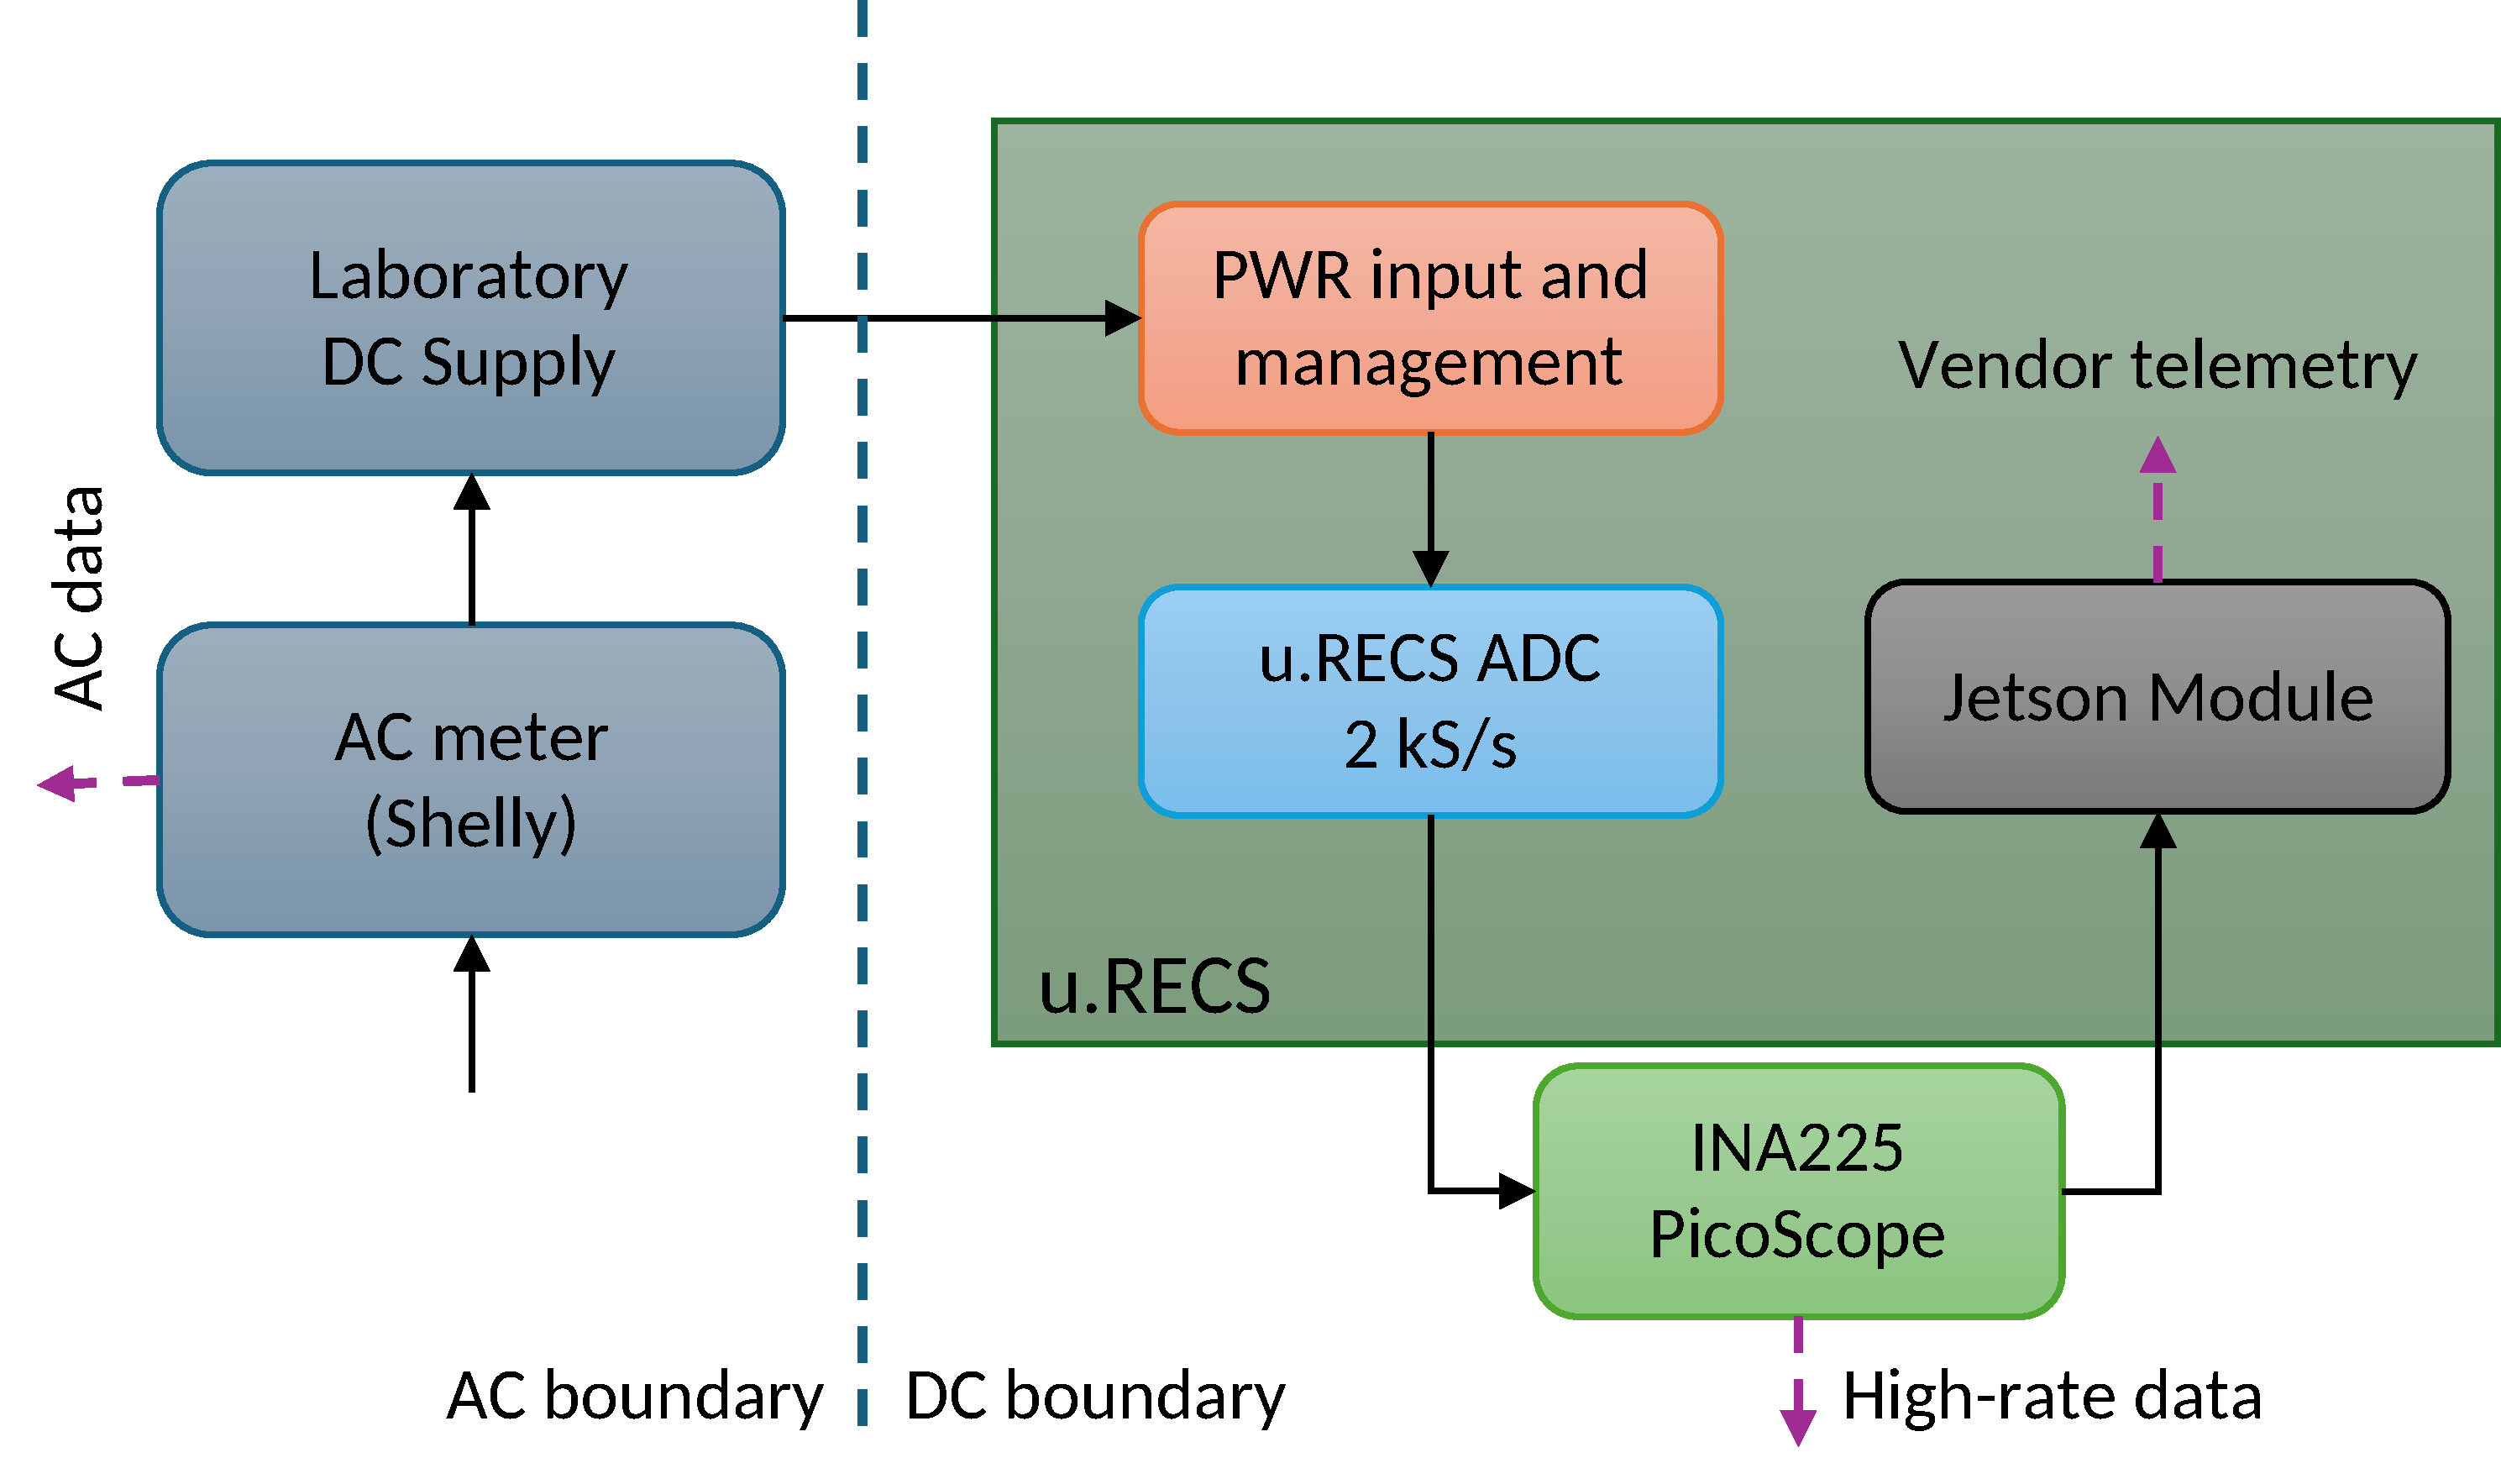
\includegraphics[width=.90\textwidth]{measurement_boundaries.pdf}
\caption{Electrical boundaries of the measurement setup. External and \urecs{} acquisition observe the selected DC input; vendor telemetry covers its reported rails, while the AC observation includes the supply and auxiliary loads. The diagram shows the Jetson configuration used here.}
\label{fig:setup}
\end{figure}

The external DC setup uses a 20-m$\Omega$ shunt, INA225 amplifier and PicoScope~4224A, streaming at up to 5~MS/s. Its nominal differential current-path bandwidth is approximately 77~kHz; the voltage-input bandwidth is 20~MHz. u.RECS uses a nominally equivalent analogue path with an ADS7953 12-bit ADC at 2~kS/s. Jetson INA3221 and the approximately 1-S/s Shelly Plus Plug S provide additional observations. The paired-scope study adds a Tektronix TCP0030A current-probe acquisition path and retains each path's recorded calibration and voltage treatment \cite{energyResults2026}.

Calibration separates gain and offset errors from workload-dependent effects. Both shunt-based current paths are calibrated against an EA-EL~9080-60~DT electronic load and a Fluke~179 reference over 36 load settings spanning 0--3.5~A. An endpoint gain/offset fit is checked in a separate verification sweep. The maximum absolute relative deviations at the nonzero settings are 2.0\% for PicoScope and 0.44\% for \urecs{} \cite{wachsmuth2026thesis}. These checks establish the static calibration basis; they are not an absolute dynamic-power uncertainty bound. Full-precision coefficients, verification results and ADC characterisation are documented in the accompanying methods and source package.

For the paired-scope study, both paths use the same load-dependent voltage model, $\widehat P=I\widehat V(I)$, with linear $\widehat V$ characterised over 0--3.5~A. Samples outside that range are extrapolated, not clipped. The Tektronix YOLO-FP32 series additionally uses a workload-specific current-offset correction, so its absolute level is not an independent agreement test. The duration and meter study retains its setup-derived voltage scaling for \urecs{} and empirical scaling for Shelly. The latter is therefore a scaled AC estimate, not raw wall-socket power. Coefficients and their provenance remain explicit in the archive \cite{energyResults2026}.

\begin{table}[htbp]
\centering\small
\caption{Experiments and their roles. Numerical windows and grid offsets reuse the same recordings; they do not increase the number of physical executions. Workload configurations and inclusion rules are documented in the accompanying methods and result archive.}
\label{tab:workloads}
\begin{tabularx}{\textwidth}{@{}L{.22\textwidth}Y@{}}
\toprule
Experiment & Question and coverage \\
\midrule
Same-trace reconstruction & Isolate rate and interval effects: six Jetson workloads, 59 paired executions and 118 traces at 5~MS/s; nine intervals from 20~ms to 10~s. \\
Long-window FP16 & Contrast energy with fluctuation coverage: 15 GEMM-FP16 recordings, each with a 104-s energy interval and same-record active/idle segments. \\
Direct acquisition & Assess execution, interval and meter effects: eight Jetson workloads in rate sweeps and seven in 5--600-s duration requests; 15 planned repetitions per setting. Meter comparison at 300~s uses 15 executions per workload. \\
Rate-order control & Check acquisition-rate effects with work held fixed: 12 GEMM-FP16 runs, six per rate, each completing 250 queries; order balanced across two sessions. \\
\bottomrule
\end{tabularx}
\end{table}

The paired-scope workloads are GEMM and YOLO in FP32 and INT8, Gemma3-4B and ResNet-50 FP32. Each has ten paired executions except ResNet-50, which has nine. The direct Jetson study covers TensorRT GEMM/YOLO in FP32, FP16 and INT8, variable-activity YOLO and Gemma3-12B via Ollama. FP32 labels permit TensorRT's TF32 option. Variable YOLO alternates activity and pauses, providing a contrast to the six continuous GEMM/YOLO cases. Workload scripts and available configuration details are retained with the results.

Direct sampling spans 50~S/s--5~MS/s at 27 rates, except Jetson YOLO-FP32 with 26. Jetson GEMM/YOLO rate runs request fixed engine iteration counts; the LLM runs to completion. Duration measurements use time-controlled execution. The Jetson duration/meter comparison acquires PicoScope and \urecs{} at 2~kS/s. Available series settings are archived; missing YOLO input/batch metadata limit exact workload replication \cite{wachsmuth2026thesis,energyResults2026}.

\section{Measurement and Analysis}
\label{sec:method}
\subsection{Define the energy interval before comparing rates}
Energy and mean power are evaluated over the actual interval $[t_0,t_1]$:
\begin{equation}
 E=\int_{t_0}^{t_1}P(t)\,\mathrm{d}t,
 \qquad \overline P=E/(t_1-t_0).
 \label{eq:energy}
\end{equation}
Here $P$ is measured or model-derived power as specified for the series. We use trapezoidal integration and retain telemetry timestamps. Requested duration controls the benchmark command, not the denominator of mean power. This prevents a short detected load interval from being averaged over a longer nominal runtime.

The load-window detector uses time-weighted 100-ms power bins. It checks that activity is distinguishable from edge-region idle variation and requires at least 200~ms above a threshold halfway between idle and high-load power. The interval spans the first to last qualifying activity, retaining internal pauses. Thresholds at 40\% and 60\% provide a sensitivity check. All finite, positive-duration results are retained; windows are never adjusted to obtain a preferred duration or energy result. The exact detector and settings are in the public methods archive \cite{energyResults2026}.

For repeated acquisitions, we report energy CV and differences between rate-group means separately. CV is the population standard deviation divided by the mean. Each group's deviation is measured against the equally weighted mean of all rate-group means. Meter comparisons at a common 300-s request instead pair run IDs and calculate $d_r=100(\overline P_{s,r}/\overline P_{\mathrm{Pico},r}-1)$ for each sensor $s$. We report the median and empirical 5th--95th percentiles of these signed pair differences, not a ratio of group medians or a confidence interval. Each meter retains its own integration window; pairing identifies the execution, not identical temporal or electrical boundaries.

\subsection{Test slower sampling on the same execution}
\label{sec:common}
To isolate sampling from execution variability, we reconstruct lower-rate observations from each native 5-MS/s power trace while keeping its integration endpoints fixed. The reference is that same trace's native integral, not a different execution or the other instrument. Candidate rates span 50~S/s--160~kS/s over nine durations from 20~ms to 10~s. Up to 16 windows per duration and 64 sampling-grid offsets per rate test sensitivity to when the sampling clock meets the workload. Eligible cases require at least four target-rate samples.

The primary reconstruction adds no target-rate filtering. It interpolates the recorded power onto the shifted grid and preserves the reference endpoints. Its relative error is
\begin{equation}
 \epsilon=100\frac{|E_{\mathrm{reconstructed}}-E_{\mathrm{reference}}|}
 {E_{\mathrm{reference}}}.
 \label{eq:error}
\end{equation}
For each recording, we take Q95 over window/offset errors, then Q95 over recordings within a workload and acquisition path. This \emph{hierarchical Q95} gives physical executions equal standing despite many numerical cases. The reported envelope is its largest value across the six workloads and two paths. All quantiles use linear interpolation. A fixed-rate pass answers whether that rate meets the tolerance; a \emph{persistent minimum} additionally requires every higher eligible tested rate to pass. This distinction matters because reconstruction error need not decrease monotonically with rate.

A matched comparison reconstructs the same windows after intermediate reduction to 1~MS/s, against the same native reference. It tests sensitivity to the processing path rather than redefining the main result. The separate FP16 energy experiment uses all 15 recordings, 104-s intervals, three rates (50, 85 and 2,000~S/s) and 64 offsets per recording. Its Q95 pools the recording/offset errors. These empirical criteria describe the tested data and grid, not bounds on all future executions.

\subsection{Ask separately which fluctuations remain observable}
\label{sec:psd-method}
Spectral coverage measures something different from energy error: how much measured fluctuation variance lies below a candidate rate's Nyquist frequency. For FP16, we compare equal-length 4-s active and pre-run idle segments from each of the 15 recordings. After separate mean removal, Welch estimation at 1~MS/s uses one-second Hann windows and 50\% overlap, giving seven segments in each interval.

We subtract idle from active PSD and set negative differences to zero. The resulting \emph{positive excess} describes measured fluctuations above idle. For each recording, the fraction of its area below half the candidate rate is the spectral coverage. A rate meets a coverage target when the empirical fifth percentile across recordings reaches that target. Unlike the integral in Equation~\ref{eq:energy}, PSD area is variance in W$^2$, not energy in joules. Checks with unequal active/idle lengths and split-idle comparisons assess the estimator's sensitivity; clipping is not presented as a noise-bias correction.

Native 5-MS/s spectra complement this FP16 example by testing acquisition-path and workload dependence. Paired Jetson spectra use 10-s active intervals and separate idle records. The precise aggregation orders are documented with the outputs. A 250-MS/s Tektronix check finds less than 0.02\% of measured spectral variance above the 5-MS/s Nyquist limit for all six Jetson workloads; GEMM-FP32 uses an active-only diagnostic, the others an idle-subtracted one \cite{energyResults2026}. This supports the reference rate for the observed signals without removing the instruments' analogue response.

\subsection{Validate the acquisition protocol, not just reconstruction}
\label{sec:control-method}
Same-trace reconstruction cannot reveal variation introduced by rerunning a workload. We therefore compare direct rate groups, requested durations and paired meters. A fixed record-relative 20--80-s check uses 225 recordings from five workloads at 2~kS/s, 250~kS/s and 5~MS/s, keeping outer load-window detection out of that comparison.

The rate-order control holds the FP16 engine, 250 completed queries and \texttt{--useSpinWait} fixed, with 120-s pauses between processes. Two complementary six-run sessions place each rate at every sequence position across sessions. A linear model estimates the 5-MS/s-minus-2-kS/s difference while accounting for session and position. Its 95\% $t$ interval has four residual degrees of freedom and assumes additive session differences and common position effects. This control asks whether a rate difference is resolved under a fixed-work protocol; it is not an equivalence test.

\section{Results}
\subsection{RQ1: Longer intervals make low-rate energy measurement viable}
\label{sec:energy-results}
The energy result depends strongly on how long the workload is integrated. At a fixed 2~kS/s, the six-workload envelope falls from about 11\% for 20-ms intervals to \FinalScopeTen\% for 10-s intervals (Figure~\ref{fig:common-duration}). The empirical 1\% criterion is met at the tested 2-, 5- and 10-s intervals; the 0.5\% criterion is met at 10~s. A rate that is inadequate for short activity can therefore be sufficient for its accumulated energy.

\begin{figure}[htbp]
\centering
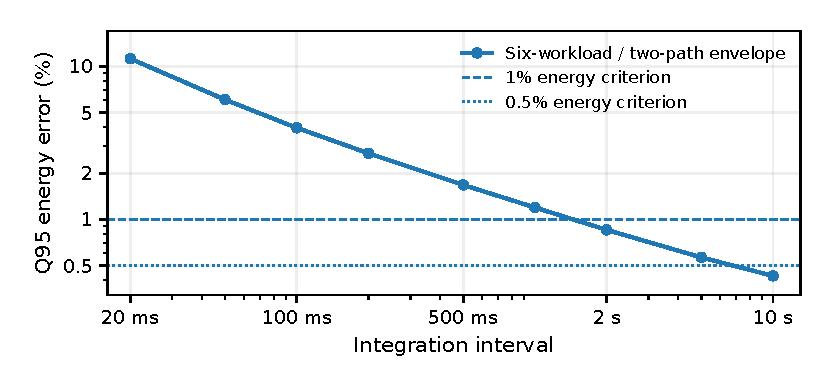
\includegraphics[width=.88\textwidth]{scope_native_energy.pdf}
\caption{Energy reconstruction at a fixed 2~kS/s from native 5-MS/s traces, without additional target-rate filtering. Each point is the largest hierarchical Q95 across six Jetson workloads and two acquisition paths, not the largest individual error. Lines connect tested durations; they do not establish guarantees between them.}
\label{fig:common-duration}
\end{figure}
\begin{table}[htbp]
\centering\small
\caption{Rate and interval must be chosen together. Native-reconstruction envelope at 2~kS/s and persistent minima for which that rate and every higher eligible tested rate pass. A dash means not reached within the tested grid up to 160~kS/s.}
\label{tab:common-duration}
\begin{tabular}{@{}rrrr@{}}
\toprule
Interval & Q95 error at 2 kS/s (\%) & $f_{\min}(1\%)$ & $f_{\min}(0.5\%)$ \\
\midrule
20 ms & 11.23 & 160 kS/s & --- \\
50 ms & 6.05 & 80 kS/s & --- \\
100 ms & 3.96 & 80 kS/s & 160 kS/s \\
200 ms & 2.70 & 80 kS/s & 80 kS/s \\
500 ms & 1.68 & 16 kS/s & 80 kS/s \\
1 s & 1.19 & 16 kS/s & 80 kS/s \\
2 s & 0.85 & 16 kS/s & 16 kS/s \\
5 s & 0.56 & 1.2 kS/s & 16 kS/s \\
10 s & 0.43 & 680 S/s & 16 kS/s \\
\bottomrule
\end{tabular}

\end{table}

Table~\ref{tab:common-duration} also explains why a single successful rate is not a monotonic sampling rule. At 2~s, 2~kS/s gives \FinalScopeTwo\% Q95 error, yet 9.4~kS/s reaches about 1.02\%. The persistent 1\% minimum is consequently 16~kS/s. At 10~s, a similar distinction holds for the 0.5\% criterion. The matched 1-MS/s-processing comparison preserves the fixed-2-kS/s passes, but changes some persistent minima. Rate recommendations therefore need both the reconstruction method and the decision rule; integral preservation alone is insufficient.

The long-window FP16 case makes the same point more sharply. Across 15 recordings, even 50~S/s gives only \FinalFPFifty\% pooled Q95 error over 104~s. Individual cases can still exceed 1\%; at 85~S/s all 960 tested recording/offset cases remain below it. At 2~kS/s, Q95 is \FinalFPTwoK\%. These are reconstruction results for a long interval, not claims that a 50-S/s instrument reproduces the waveform.

\begin{table}[htbp]
\centering
\small
\caption{Jetson direct rate sweeps: largest repeat variation and group deviation across rates. Group deviation compares each rate-group mean with the equally weighted mean of all rate-group means. All finite results are retained.}
\label{tab:rate-results}
\begin{tabular}{@{}lrrR{.23\textwidth}R{.23\textwidth}@{}}
\toprule
Workload & Rates & Runs & Largest repeat variation (CV) & Largest group deviation \\
\midrule
GEMM-FP32 & 27 & 405 & 0.37\% & 0.40\% \\
GEMM-FP16 & 27 & 405 & 0.73\% & 2.08\% \\
GEMM-INT8 & 27 & 405 & 0.63\% & 1.69\% \\
YOLO-FP32 & 26 & 390 & 0.41\% & 0.89\% \\
YOLO-FP16 & 27 & 405 & 0.44\% & 0.25\% \\
YOLO-INT8 & 27 & 405 & 0.73\% & 0.31\% \\
Gemma3-12B & 27 & 405 & 0.58\% & 1.66\% \\
Variable YOLO & 27 & 405 & 0.49\% & 0.56\% \\
\bottomrule
\end{tabular}
\end{table}

Direct acquisitions add a second source of variation: the executions themselves. Table~\ref{tab:rate-results} separates repeatability at one rate from differences between rate groups. Jetson GEMM-FP16 has no more than 0.73\% within-rate CV, yet its largest group deviation is \FPsixteenMaxBetween\%. Repeatable groups can thus produce different energy totals. The fixed 20--80-s analysis also retains differences between rate groups, so the outer load-window detector cannot explain the whole effect.

\begin{table}[htbp]
\centering\small
\caption{Fixed-work acquisition-rate control: six runs per rate. Changes are 5~MS/s minus 2~kS/s, adjusted for session and sequence position and expressed relative to the 2-kS/s mean. Intervals are 95\% $t$ intervals of the fitted model, not equivalence bounds.}
\label{tab:controlled}
\begin{tabular}{@{}lrrrr@{}}
\toprule
Quantity & 2 kS/s mean & 5 MS/s mean & Change (\%) & 95\% interval (\%) \\
\midrule
PicoScope load power (W) & 35.04 & 35.01 & -0.06 & [-0.18, +0.06] \\
Jetson input power (W) & 34.17 & 34.18 & +0.01 & [-0.07, +0.09] \\
Time for 250 queries (s) & 117.42 & 117.38 & -0.03 & [-0.17, +0.11] \\
\bottomrule
\end{tabular}
\end{table}

Holding completed work and acquisition order under control substantially narrows the comparison (Table~\ref{tab:controlled}). The adjusted PicoScope load-power difference is about $-0.06\%$, with a 95\% interval of approximately $[-0.18\%,+0.06\%]$. Neither it nor the input-telemetry and query-time intervals resolves a rate effect under the model. This is consistent with accurate energy reconstruction at 2~kS/s, while also showing why a direct rate sweep alone cannot isolate a sampling mechanism.

\subsection{RQ2: Preserving energy does not preserve fluctuations}
The FP16 spectrum reveals what the low energy error does not tell us. At 2~kS/s, only about 4\% of measured positive excess fluctuation variance lies below Nyquist, despite the small 104-s energy error. By contrast, 125 and 160~kS/s meet the 95\% and 99\% coverage targets: their lower empirical coverage percentiles are about 97.5\% and 99.3\%, respectively (Figure~\ref{fig:jetson-psd}). The two measurement objectives differ by orders of magnitude in useful sampling rate.

\begin{figure}[htbp]
\centering
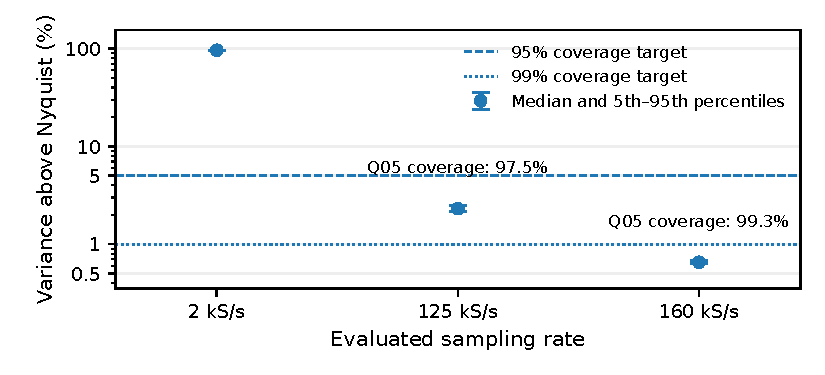
\includegraphics[width=.88\textwidth]{fp16_variance_coverage.pdf}
\caption{GEMM-FP16 fluctuation variance lying \emph{above} Nyquist at three evaluated rates, using all 15 recordings and matched active/idle Welch segments. Markers show medians and bars empirical 5th--95th percentiles. The 125-/160-kS/s observations meet 95\%/99\% coverage, respectively; no unsampled minimum is inferred.}
\label{fig:jetson-psd}
\end{figure}

The coverage conclusions also hold with longer active segments and in split-idle comparisons. Positive excess nevertheless remains a descriptive measured quantity: subtracting and clipping PSDs does not identify a noise-free workload signal. For energy benchmarking, the implication is not to require 160~kS/s everywhere. It is to avoid using a low-error energy integral as evidence that fine-grained power behaviour has been retained.

The measurement path also shapes the spectrum. Across the paired Jetson workloads, cumulative distributions differ by up to about 31 percentage points over the full recorded band, but by at most about 3 points when each is normalised within the common 77-kHz band. This contrast shows why spectral coverage must be stated for the analogue path actually used, even when long-window energy is the intended output \cite{energyResults2026}.

\subsection{RQ3: Validating the deployed measurement}
\label{sec:deployed}
The reconstruction results support low-rate integration, but not arbitrary benchmark lengths or interchangeable meters. Figure~\ref{fig:duration} first holds the DC measurement path fixed and varies the duration request. For GEMM-FP16, a 5-s request gives about 6.3\% less mean power than the 600-s group, while its median detected load interval is only 3.0~s. At a 100-s request, the six continuous workload medians are within 2\% of their 600-s references. Longer execution reduces these observed differences, but 600~s is a comparison point, not a demonstrated steady-state limit.

\begin{figure}[htbp]
\centering
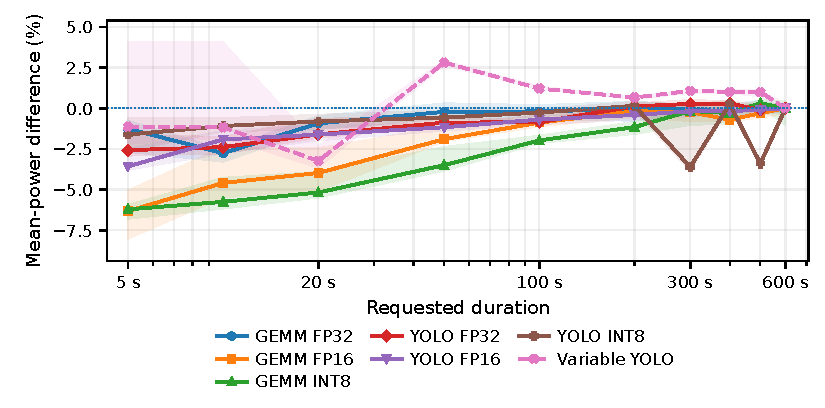
\includegraphics[width=.90\textwidth]{duration_dependence.pdf}
\caption{Jetson mean power in the actual integration interval versus requested duration. Lines show medians and shaded bands empirical 5th--95th percentiles, relative to each workload's fixed 600-s median. Bands describe run spread, not confidence intervals. The dashed curve denotes variable YOLO activity.}
\label{fig:duration}
\end{figure}

\begin{figure}[htbp]
\centering
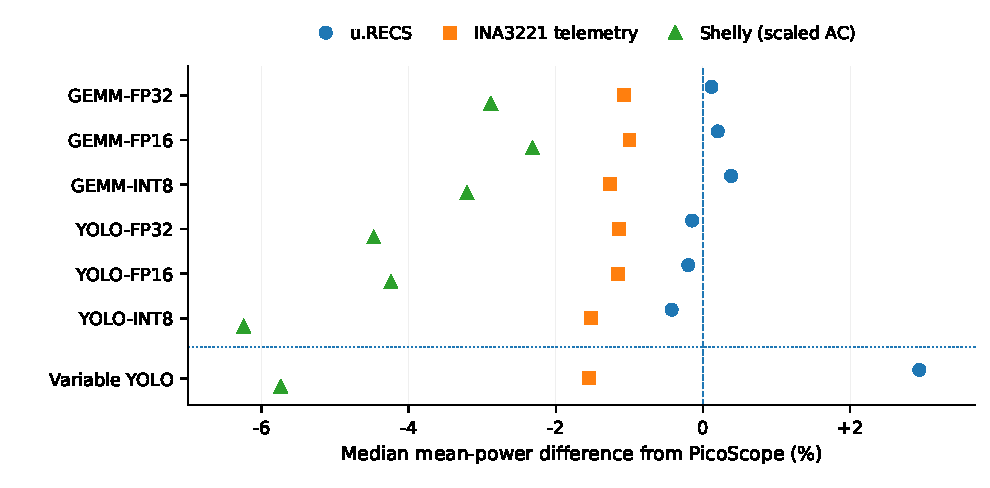
\includegraphics[width=.96\textwidth]{device_pair_medians.pdf}
\caption{Jetson at a 300-s request: median signed mean-power differences from PicoScope, using 15 paired executions per workload. Shapes distinguish the three measurement paths; the separated bottom row is variable YOLO activity. Full pair distributions remain in the artifact. Sensor-specific windows and recorded scaling are retained, so these are protocol-level comparisons rather than intrinsic meter errors.}
\label{fig:devices}
\end{figure}
At the common 300-s request, Figure~\ref{fig:devices} compares embedded sensing, input telemetry and AC observations from the same executions. The six continuous workloads show close \urecs{} agreement: every median power difference is within $\pm0.5\%$. This supports the embedded 2-kS/s implementation for these long, continuous measurements, without claiming that every individual difference is below 0.5\% or that short transients are preserved.

Input telemetry reports about 1.0--1.5\% lower mean power across the continuous workloads. Its narrow pair distributions, retained in the artifact, show that repeatability does not establish agreement with an external observation. Scaled Shelly estimates are about 2--6\% lower, with a larger workload-dependent displacement. The AC path includes the supply and auxiliary loads and uses empirical scaling: these differences compare measurement procedures, not the plug meter's intrinsic accuracy.

Variable YOLO tests whether the continuous-load agreement transfers to intermittent activity. Here the \urecs{} median difference rises to $+\ParmaVariableUrecsRounded\%$, even though the nominal acquisition rate is unchanged. The archived pair distribution remains narrow: the difference is not merely a few dispersed runs. The telemetry and scaled AC estimates remain lower than PicoScope. This is a consistent difference within the cohort, not an identified mechanism: the meters retain their own windows and calibrated response.

Together, these comparisons make deployment validation the last step of rate selection: the intended workload, integration interval and electrical boundary must be tested as well as the rate.

\FloatBarrier
\section{Practical Implications and Scope}
The results support a two-stage measurement strategy. First, use representative high-rate traces to choose a rate for a defined quantity and interval. For energy, assess reconstruction error under shifted sampling grids; for fluctuations, specify how much measured spectral variance must remain observable. Then repeat measurements at the intended acquisition rate, checking completed work, actual load spans and repeatability. This second stage catches protocol effects that numerical resampling cannot expose.

The concrete operating points make the distinction useful. A fixed 2~kS/s passes the stated energy criteria for multi-second intervals in the paired Jetson cohort, while the FP16 spectral objective calls for much higher rates. Neither result licenses arbitrarily short measurements or transfer to a different front end. Likewise, a persistent minimum should not be confused with the first rate that happens to pass: the nonmonotonic cases in Table~\ref{tab:common-duration} matter when reporting a general rate threshold.

Three limits govern interpretation. Reconstruction measures deviation from each trace's calibrated, sometimes model-derived reference; it does not establish absolute dynamic-power uncertainty. Spectral coverage retains the acquisition response and positive-excess estimator, and the 77-kHz front end is not anti-alias protection for arbitrary signals sampled at 2~kS/s. Finally, the finite Jetson cohorts support workload-specific measurement conclusions, not universal meter specifications. The 300-s comparison tests protocol-level agreement; it does not establish sensor interchangeability for short bursts.

\medskip\noindent\textbf{Reproducibility.}
The result archive is cited at a fixed repository commit \cite{energyResults2026}. It provides detailed calibration and window methods, recording inventories, full-precision result summaries and robustness evidence. The accompanying source package maps each figure and table to its inputs and regenerates the manuscript outputs from the included summaries. Raw waveform recomputation requires the original recordings and matching acquisition settings; those are not implied by availability of the compact result package.

\section{Conclusion}
The useful sampling rate depends on the measurement question. Across six Jetson workloads, 2~kS/s meets the empirical hierarchical 1\% energy criterion at the tested 2-, 5- and 10-s intervals; the long-window FP16 example passes its pooled criterion even at 50~S/s. Its 95\% and 99\% fluctuation-coverage targets are instead met at 125 and 160~kS/s. The deployed-meter comparison shows close continuous-load agreement and its limits under variable activity. Representative intervals and electrical boundaries therefore remain essential after the rate is chosen. The practical recommendation is not ``sample as fast as possible'', but \emph{choose the quantity, validate the rate, and verify the deployed measurement}.

\FloatBarrier
\clearpage
\begingroup\interlinepenalty=10000\bibliography{references}\endgroup
\end{document}
